\documentclass[11pt]{article}
\usepackage{fullpage}
\usepackage{url}
\usepackage{amsmath, graphicx}
\begin{document}
\thispagestyle{empty}
\parindent 0pt
\vfill
\large

\begin{center}
\LARGE{\bf \textsf{CS246: Mining Massive Datasets}}\\ {\bf \textsf{Homework 2}} 
\\*[4ex]
\end{center}

\section*{Answer to Question 1(a)}
Below is the proof, this proof use the properties of $M$: $\sum_iM_{ij}=\mathbf{1}$
\begin{equation*}
\begin{aligned}
    \omega(r') & = \omega(Mr)\\
    & = \sum_i\sum_jM_{ij}r_j\\
    & = \sum_jr_j\sum_iM_{ij}\\
    & = \sum_jr_j1\\
    & = \sum_jr_j\\
    & = \omega(r)
\end{aligned}
\end{equation*}

\pagebreak[4]
\section*{Answer to Question 1(b)}
\begin{equation*}
\begin{aligned}
    \omega(r') & = \omega(Mr)\\
    & = \sum_i(\sum_j\beta M_{ij}r_j+(1-\beta)/n)\\
    & = \sum_jr_j\sum_i\beta M_{ij}+\sum_i(1-\beta)/n\\
    & = \beta\sum_jr_j + (1-\beta)
\end{aligned}
\end{equation*}
In order to make $\omega(r') = \omega(r)$:
\begin{equation}
\begin{aligned}
    & \beta\sum_jr_j + (1-\beta) = \sum_jr_j\\
    & \omega(r) = \sum_jr_j = 1
\end{aligned}
\end{equation}

\pagebreak[4]
\section*{Answer to Question 1(c)}
We can divide the node into two sets one for dead nodes and the other for live nodes
\begin{equation*}
    r'_i = \beta\sum_j M_{ij}r_j + [(1-\beta)\sum_{j\in live}r_j + \sum_{j\in dead}r_j]/n
\end{equation*}
As we know for dead node: $\sum_{j\in dead} M_{ij} = \mathbf{0}$. Therefore,
\begin{equation}
\begin{aligned}
    r'_i & = \beta\sum_{j\in live} M_{ij}r_j + (1-\beta)\sum_{j\in live}r_j/n + \sum_{j\in dead}r_j/n\\
    & = \sum_{j\in live}(\beta M_{ij} + (1-\beta)/n)r_j + \sum_{j\in dead}r_j/n\\
\end{aligned}
\end{equation}
Then use above equation to prove $\omega(r') = \omega(r)$:
\begin{equation}
\begin{aligned}
    \omega(r') & = \omega(Mr)\\
    & = \sum_i\sum_{j\in live}(\beta M_{ij} + (1-\beta)/n)r_j + \sum_i\sum_{j\in dead}r_j/n\\
    & = \sum_{j\in live}r_j\sum_i(\beta M_{ij} + (1-\beta)/n) + \sum_{j\in dead}r_j1\\
    & = \sum_{j\in live}r_j + \sum_{j\in dead}r_j\\
    & = \sum_jr_j\\
    & = \omega(r)
\end{aligned}
\end{equation}

\pagebreak[4]
\section*{Answer to Question 2(a)}
$MM^T$ and $M^TM$ are symmetric.
$$(MM^T)^T = MM^T$$
$$(M^TM)^T = M^TM$$
It is obvious they are square matrix, $MM^T$ has dimension of $p \times p$ and $M^TM$ has dimenstion of $q \times q$.
Given most of the data are real number, then these matrix are real as well.

\pagebreak[4]
\section*{Answer to Question 2(b)}
Suppose $\mathbf{e}$ is an eigenvector of $M^TM$, that is:
\begin{equation*}
    M^TMe = \lambda e
\end{equation*}
Multiply both sides by $M$:
\begin{equation*}
    MM^T(Me) = M\lambda e = \lambda (Me)
\end{equation*}
Where $Me \neq \mathbf{0}$, becuase if $Me = \mathbf{0}$ then $M^TMe = \mathbf{0}$ thus $e$ cannot be eigenvector.
Therefore, we find $Me$ is a eigenvector of $MM^T$, and $\lambda$ is also the eigenvalue if $MM^T$.\\
\\
In conclusion, $MM^T$ and $M^TM$ has the same eigenvalue. Their eigenvectors are not necessarily the same.

\pagebreak[4]
\section*{Answer to Question 2(c)}
Since already approved in part a that $M^TM$ is a real, symmetric and square matrix.
Then we can apply eigenvalue decomposition of a real,symmetric and square matrix:
\begin{equation}
    M^TM = Q\Lambda Q^T
\end{equation}

\pagebreak[4]
\section*{Answer to Question 2(d)}
Apply the SVD decomposition for matrix $M$, also it is important to note that $U^TU = \mathbf{I}$
\begin{equation}
\begin{aligned}
    M^TM & = (U\Sigma V^T)^T(U\Sigma V^T)\\
    & = V\Sigma^TU^TU\Sigma V^T\\
    & = V\Sigma^T\Sigma V^T
\end{aligned}
\end{equation}

\pagebreak[4]
\section*{Answer to Question 2(e)}
\begin{enumerate}
\item
From SVD we obtain:
\begin{equation*}
    M = U\Sigma V^T
\end{equation*}
Where,
$$
U = 
\begin{pmatrix}
    &-0.27854301 & 0.5\\
    &-0.27854301 & -0.5\\
    &-0.64993368 & 0.5\\
    &-0.64993368 & -0.5
\end{pmatrix}
$$
$$
\Sigma = 
\begin{pmatrix}
    &7.61577311 & 0\\
    &0 & 1.41421356
\end{pmatrix}
$$
$$
V^T = 
\begin{pmatrix}
    & -0.70710678 & -0.70710678\\
    & -0.70710678 & 0.70710678
\end{pmatrix}
$$
\item
The eigenvalue and eigenvector for $M^TM$:
$$
Evectors = [(0.70710678, -0.70710678), (0.70710678, 0.70710678)]
$$
$$
    Evals = 58, 2
$$

\item
Based on the experiments, it is found that the eigenvector of $M^TM$ is the same for the $V$ in the SVD.
This can be proved using the result in 2d:
$$
    M^TM = V\Sigma^T\Sigma V^T
$$
Therefore, $V$ is the matrix composed by its eigenvectors.

\item
Based on the experiments, it is found that the singular value of $M$ (denote as $s$) and eigenvalue of $M^TM$ (denote as $\lambda$):
\begin{equation}
    s^2 = \lambda
\end{equation}
It is obvious to prove: the singular value of $M$ are on the diagonal of $\Sigma$ while the eigenvalue of $M^TM$ are on the diagonal of $\Sigma^T\Sigma$.

\end{enumerate}

\pagebreak[4]
\section*{Answer to Question 3(a)}
5 nodes with top page rank: [53, 14, 40, 1, 27]\\
5 nodes with lowest page rank: [85, 59, 81, 37, 89]

\pagebreak[4]
\section*{Answer to Question 3(b)}
5 nodes with top hubbiness: [59, 39, 22, 11, 58]\\
5 nodes with top hubbiness: [9, 35, 15, 95, 53]\\
5 nodes with top authority: [66, 40, 27, 53, 1]\\
5 nodes with top authority: [54, 33, 24, 67, 50]

\pagebreak[4]
\section*{Answer to Question 4(a)}
Percentage change:\\
Euclidean c1.txt 0.26398863292043157\\
Euclidean c2.txt 0.7525973243724743\\
\\
It is found that by initializing with c2.txt the cost is smaller than random initialization.
Random initialization seems get trapped in its local optimal.

\begin{figure}[h]
\center
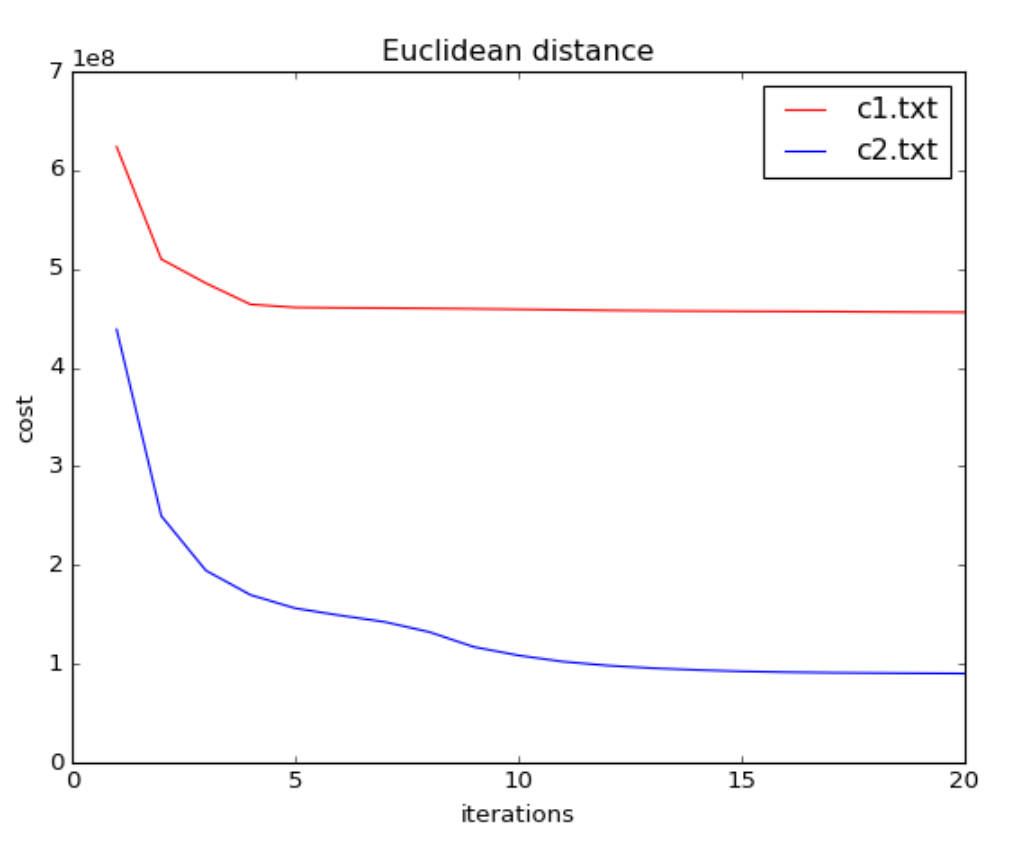
\includegraphics[scale=0.7]{Euclidean.png}
\caption{Euclidean Distance}
\end{figure}


\pagebreak[4]
\section*{Answer to Question 4(b)}
Percentage change:\\
Manhattan c1.txt 0.16884444201690121\\
Manhattan c2.txt 0.49967689555556216\\
\\
From the figure below we can find the result is different from previous part. 
When using different distance measure, the ideal clustering is changed. Therefore c2.txt may not be closer to the ideal clustering than c1.txt.

\begin{figure}[h]
\center
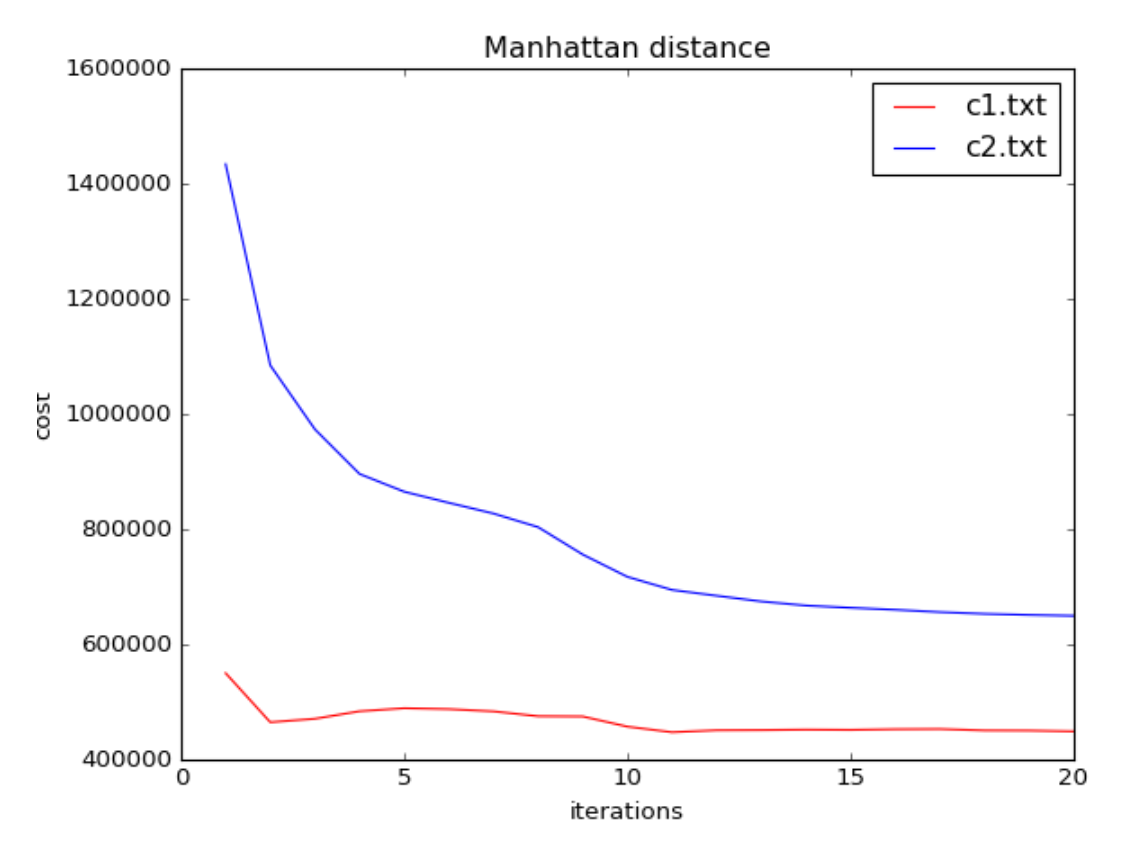
\includegraphics[scale=0.7]{Manhattan.png}
\caption{Manhattan Distance}
\end{figure}

\pagebreak[4]
\begin{center}
\LARGE{\bf \textsf{Cover Sheet}} \\*[4ex]
\end{center}

\textbf{Assignment Submission } Fill in and include this cover sheet with each of your assignments. Assignments are due at 11:59pm. All students (SCPD and non-SCPD) must submit their homeworks via GradeScope (\url{http://www.gradescope.com}). Students can typeset or scan their homeworks. Make sure that you answer each question on a separate page. Students also need to upload their code at \url{http://snap.stanford.edu/submit}. Put all the code for a single question into a single file and upload it. Please do not put any code in your GradeScope submissions. 
\\
\\
\textbf{Late Day Policy } Each student will have a total of {\em two} free late periods. {\em One late period expires at the start of each class.} (Homeworks are usually due on Thursdays, which means the first late periods expires on the following Tuesday.) Once these late periods are exhausted, any assignments turned in late will be penalized 50\% per late period. However, no assignment will be accepted more than {\em one} late period after its due date. 
\\
\\
\textbf{Honor Code } We strongly encourage students to form study groups. Students may discuss and work on homework problems in groups. However, each student must write down their solutions independently i.e., each student must understand the solution well enough in order to reconstruct it by him/herself.  Students should clearly mention the names of all the other students who were part of their discussion group. Using code or solutions obtained from the web (github/google/previous year solutions etc.) is considered an honor code violation. We check all the submissions for plagiarism. We take the honor code very seriously and expect students to do the same. 

\vfill
\vfill

{\Large
\textbf{Your name:} \hrulefill \\
\textbf{Email:} \underline{\hspace*{7cm}} \textbf{SUID:} \hrulefill\\*[2ex] }
Discussion Group (People with whom you discussed ideas used in your answers): \\\\\\
On-line or hardcopy documents used as part of your answers: \\\\\\
\vfill

\vfill

I acknowledge and accept the Honor Code.\\*[3ex]
\bigskip
\textit{(Signed)}\hrulefill
% If you are not printing this document out, just type your initials above

\vfill
\vfill

\end{document}

